% =====================================================================
%  Chapitre 1 -- Donnees sequentielles
%  Partie b : embeddings, ordre, padding, dependances
% =====================================================================

\begin{frame}{L'embedding : un mot devient un vecteur}
\begin{columns}[t]
\begin{column}{0.50\textwidth}
\centering
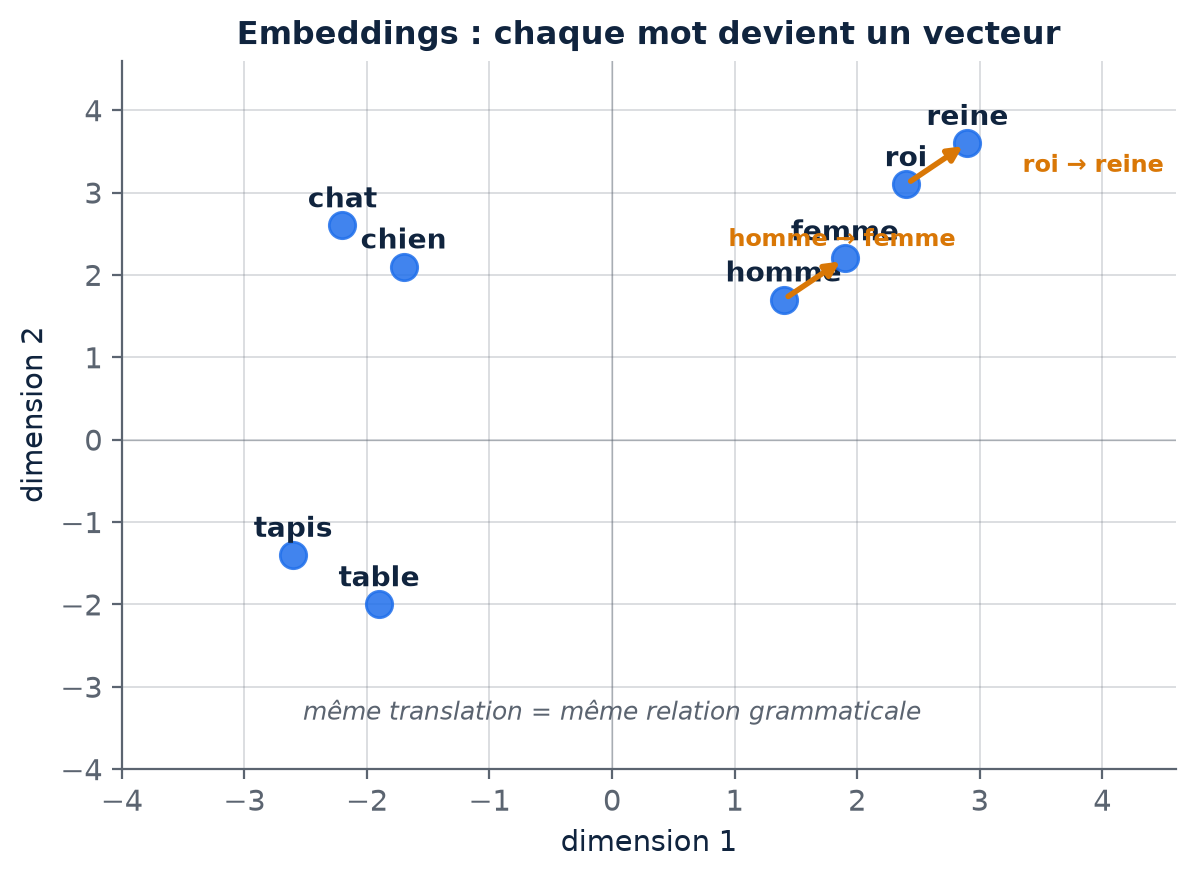
\includegraphics[width=\textwidth]{r02_embeddings.png}
\end{column}
\begin{column}{0.46\textwidth}
\begin{itemize}
  \item Chaque mot du vocabulaire reçoit un vecteur de dimension $d$
  (par exemple $d = 100$).
  \item Ces vecteurs sont \textbf{appris} pendant l'entraînement : les mots qui
  apparaissent dans des contextes voisins finissent voisins.
  \item Une relation grammaticale peut devenir une \textbf{translation} dans
  l'espace.
\end{itemize}
\begin{kbox}[Vocabulaire]
\textbf{Embedding} = table de correspondance
$\text{identifiant} \to \mathbb{R}^{d}$, apprise comme une couche du réseau.
\end{kbox}
\end{column}
\end{columns}
\end{frame}

\begin{frame}[fragile]{En PyTorch : cinq lignes}
\begin{columns}[t]
\begin{column}{0.52\textwidth}
\begin{codebox}[Tokenizer et embedding]
\begin{lstlisting}
import torch, torch.nn as nn

vocab = {"<pad>": 0, "le": 1, "chat": 2,
         "dort": 3, "sur": 4, "tapis": 5}
ids = torch.tensor([vocab[m] for m in
                    "le chat dort".split()])
print(ids)          # tensor([1, 2, 3])

emb = nn.Embedding(6, 4)
print(emb(ids).shape)   # (3, 4)
\end{lstlisting}
\end{codebox}
\end{column}
\begin{column}{0.44\textwidth}
\begin{itemize}
  \item L'identifiant $2$ devient un vecteur de 4 nombres.
  \item Une phrase de 3 mots devient une \textbf{matrice} $3 \times 4$.
  \item Le tenseur d'entrée d'un réseau séquentiel est donc
  $(\text{lot}, \text{longueur}, d)$.
\end{itemize}
\begin{wbox}[Le 0 du padding]
Réserver l'indice 0 pour le padding est une convention : son embedding
sera neutralisé par le masque.
\end{wbox}
\end{column}
\end{columns}
\end{frame}

\begin{frame}{L'ordre porte le sens}
\begin{center}
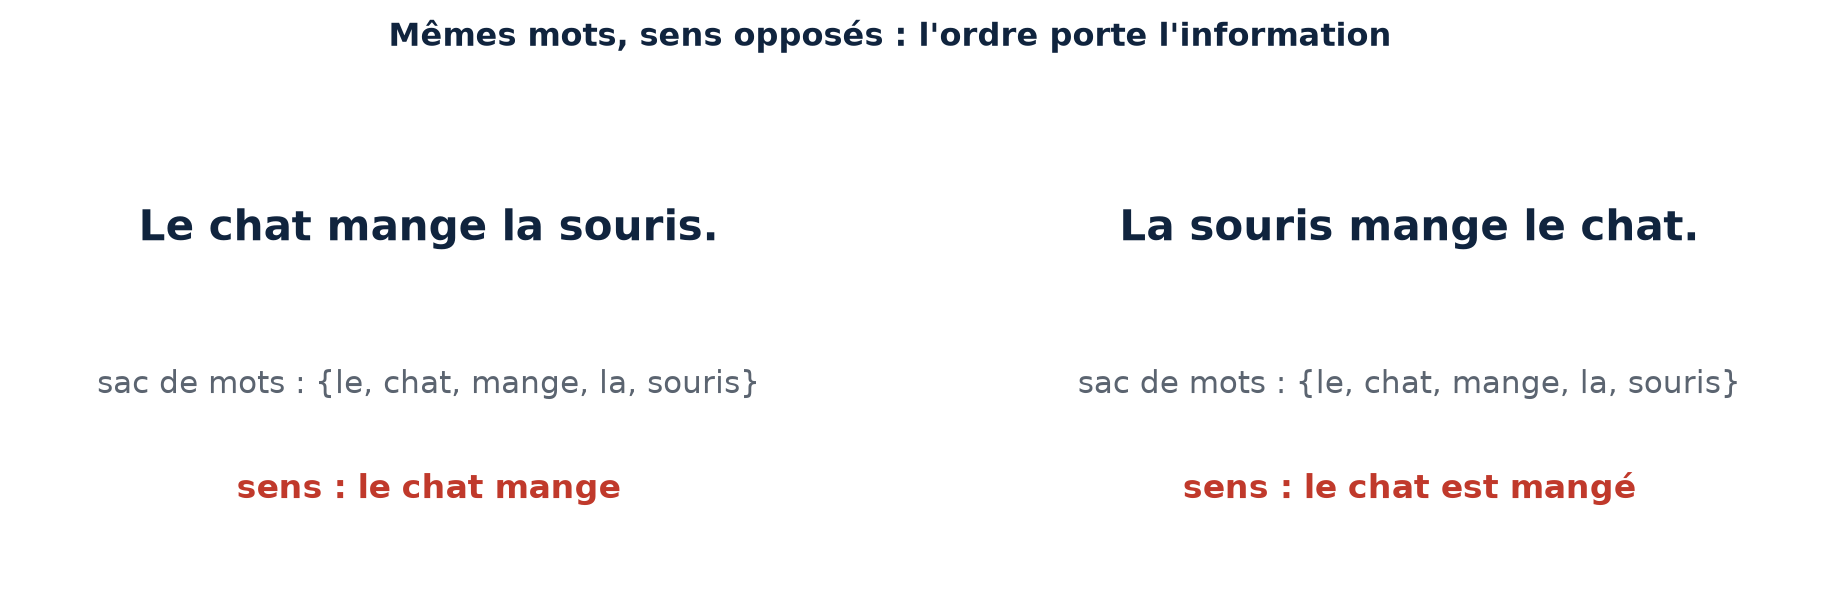
\includegraphics[width=0.9\textwidth]{r03_ordre_compte.png}
\end{center}
\vspace{1mm}
\begin{solbox}[Conclusion]
Un modèle qui additionne les embeddings des mots (sac de mots) confond ces
deux phrases. \textbf{Le traitement doit être ordonné.}
\end{solbox}
\end{frame}

\begin{frame}{Des longueurs variables dans un même lot}
\begin{center}
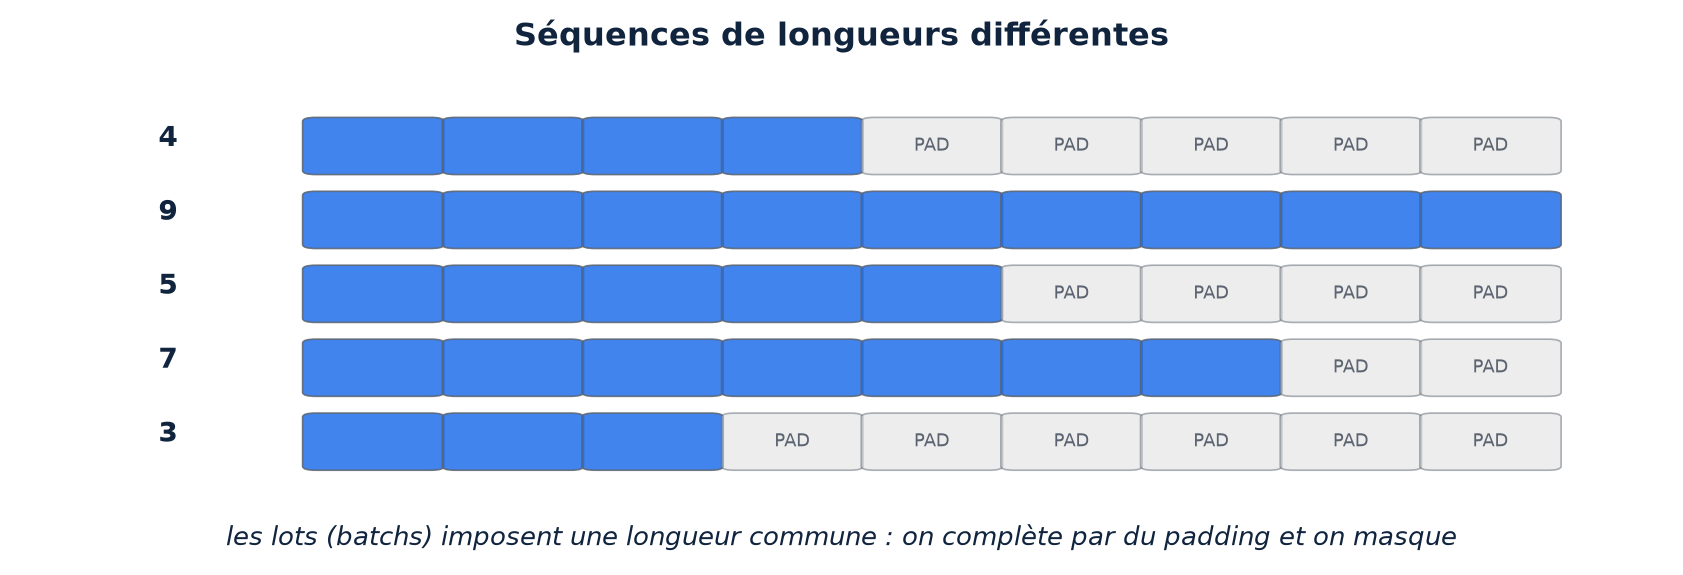
\includegraphics[width=0.9\textwidth]{r04_padding.png}
\end{center}
\vspace{1mm}
\begin{itemize}
  \item On complète avec un \textbf{token de padding} (indice 0).
  \item On fournit au réseau un \textbf{masque} : les positions de padding ne
  contribuent ni à la décision ni à la perte.
\end{itemize}
\begin{wbox}[Le piège classique]
Oublier le masque fausse les moyennes : les phrases courtes pèsent autant
que les longues, et le modèle apprend du bruit.
\end{wbox}
\end{frame}

\begin{frame}{Le vrai obstacle : les dépendances à distance}
\begin{center}
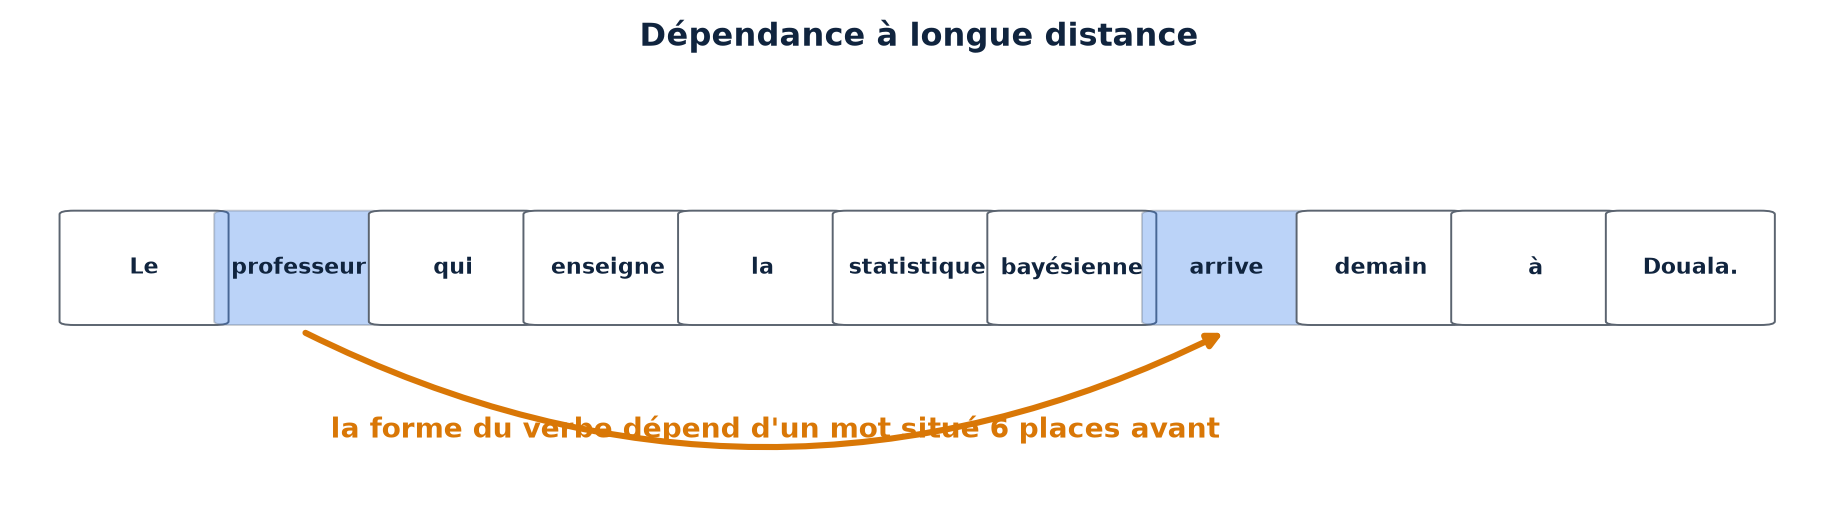
\includegraphics[width=0.94\textwidth]{r05_dependance_distance.png}
\end{center}
\vspace{1mm}
\begin{kbox}[Six places avant]
Ici, « arrive » s'accorde avec « professeur » situé 6 mots avant. Un réseau qui
ne voit qu'une fenêtre courte ne peut pas établir ce lien.
\end{kbox}
\end{frame}

\begin{frame}{Et le CNN, alors ?}
\begin{columns}[t]
\begin{column}{0.52\textwidth}
\centering
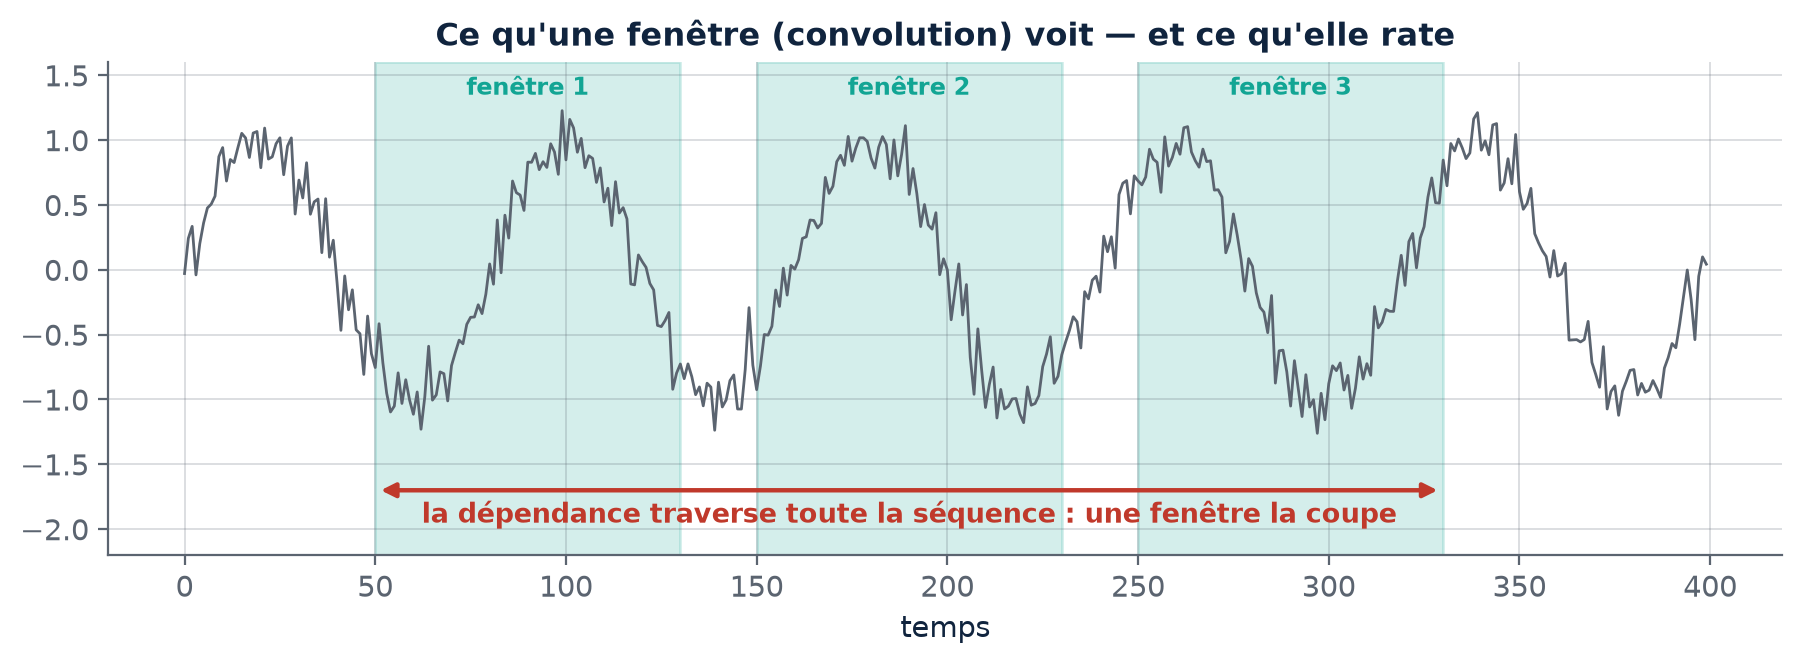
\includegraphics[width=\textwidth]{r06_fenetre_insuffisante.png}
\end{column}
\begin{column}{0.44\textwidth}
\begin{itemize}
  \item Une convolution 1D \textbf{peut} traiter du texte : elle voit des
  n-grammes.
  \item Mais pour relier deux points éloignés, il faut empiler les couches ---
  ou beaucoup de filtres.
  \item Et la longueur variable reste malcommode.
\end{itemize}
\begin{kbox}[Ce qu'il faut]
Un mécanisme qui \textbf{transporte} l'information d'un pas au suivant ---
parce que le réseau \textbf{conserve un état}.
\end{kbox}
\end{column}
\end{columns}
\end{frame}

\begin{frame}{Quiz 1 --- le terrain de jeu}
\begin{qbox}[Question 1]
Un embedding de dimension 100 pour un vocabulaire de 20 000 mots représente :
\begin{itemize}
  \item[(a)] 20 000 paramètres \quad (b) 2 000 000 \quad (c) 100
\end{itemize}
\end{qbox}
\begin{qbox}[Question 2]
Une phrase de 12 mots avec des embeddings de dimension 64 est un tenseur de forme :
\begin{itemize}
  \item[(a)] $(12,)$ \quad (b) $(12, 64)$ \quad (c) $(64, 64)$
\end{itemize}
\end{qbox}
\begin{qbox}[Question 3]
Que fait le masque sur une position de padding ?
\begin{itemize}
  \item[(a)] Il remet le mot à zéro \quad (b) Il retire la position de la décision
  et de la perte \quad (c) Il allonge la séquence
\end{itemize}
\end{qbox}
\begin{solbox}[Réponses]
\textbf{1.} (b) : $20\,000 \times 100$ poids, plus rien d'autre. \quad
\textbf{2.} (b) : longueur × dimension. \quad
\textbf{3.} (b) : c'est le masque, pas la mise à zéro seule, qui compte.
\end{solbox}
\end{frame}

\begin{frame}{À retenir et TP}
\begin{kbox}[Les trois idées du chapitre 1]
\begin{enumerate}
  \item Une donnée séquentielle est une liste \textbf{ordonnée} de longueur libre.
  \item Le texte devient un tenseur : tokens $\to$ identifiants $\to$ embeddings.
  \item Ordre et dépendances à distance exigent un mécanisme \textbf{récurrent} :
  un état qui se transporte.
\end{enumerate}
\end{kbox}
\vspace{1.5mm}
\begin{abox}[TP1 : \file{notebooks/TP1_embeddings_sequences.ipynb}]
Construire le vocabulaire, indexer, plonger, padder et masquer --- sur un petit corpus
de critiques. Durée conseillée : \textbf{1 h 30} · barème : \textbf{10 points}.
\end{abox}
\end{frame}
